\documentclass{book}
\usepackage[spanish]{babel}
\usepackage[utf8]{inputenc} 
\usepackage[T1]{fontenc}
\usepackage{lmodern}
\usepackage{graphicx}
\usepackage{amsmath}
\usepackage{xcolor} 
\usepackage{verbatim} 
\usepackage{enumerate} % enumerados
\usepackage{svg}

%\usepackage[natbibapa]{apacite}
%\usepackage[hyperpageref]{backref}
%\usepackage[alf]{abntex2cite}

\begin{document}
%\chapter{Introdución}
%	\section{Motivación}
%	\section{Planteamiento del problema}
%	\section{Hipótesis}
%	\section{Objetivos}
%	\section{Descripción del documento}
\chapter{Antecedentes}
\section{Robots bípedos}
\subsection{Conceptos básicos}
Un robot con piernas es un robot móvil que debe tener un cuerpo, al menos una pierna (extremidad inferior) y un número arbitrario de brazos (extremidades superiores). Generalmente sus piernas deben tener un actuador final con el cual apoyarse e impusarse  y sus brazos, un actuador para manipular objetos\cite{siciliano2016springer}. Por lo tanto, se puede deducir que un \textit{robot bípedo} es un robot con dos piernas las cuales usa para moverse, de forma similar al caminado.
\\

Entre los \textit{robots bípedos} más conocidos se encuentran los \textit{robots humanoides} (figura \ref{fig:humanoids}) que poseen las siguientes características:

\begin{itemize}
\item Tienen la apariencia y forma de un ser humano.
\item Pueden caminar y moverse como un ser humano.
\item Pueden interactuar con humanos usando reconocimiento de voz y de imágenes.
\end{itemize}
\textcolor{red}{Aquí podrías citar al rulebook de la categoría de humanoides, donde además de los puntos que enlistas, también mencionan que debe ser cinemáticamente equivalente a un ser humano (es decir, la rodilla por ejemplo no debe poder doblarse hacia atrás)}

Uno de los mayores retos a la hora de diseñar y modelar a los robot bípedos es su movimiento. A comparación de otros robots móviles, los robots con piernas tienden a tener un mayor número de grados de libertad en sus extremidades y estos deben estar muy bien coordinados para no hacer caer al robot. 
\\
\textcolor{red}{En lugar de usar textbf, usa subsubsection* (el asterisco pone el título sin número)}
%\textbf{Características para el diseño de un robot con piernas}				
\subsubsection*{Características para el diseño de un robot con piernas}
\begin{itemize}
\item \textbf{Tipo de marcha:} Es el patrón de movimientos de piernas del robot (caminata).

\item \textbf{Biomímesis:} Es el diseño de algunos robots para imitar la estructura mecánica de un ser vivo de tal manera que sea tan precisa como se pueda.

\item \textbf{Bioinspiración mecánica:} Es el diseño que sirve para reproducir la robustez y versatilidad de la locomoción de animales, algunos diseñadores prestan más atención en la dinámica esencial de la locomoción que en la mecánica.

\item \textbf{Simplicidad mecánica:} Con esto se pretende usar el menor número de actuadores posibles para cumplir sólo con las tareas realizadas.

\item \textbf{Espacio de trabajo de la extremidad: } Señala que una extremidad debería tener al menos 3GDL para moverse libremente en el espacio. Para que se pueda tener una arbitraria orientación en el efector final en un espacio 3-D se debe contar con almenos 6GDL.

\end{itemize}

\begin{figure}
	\centering		
	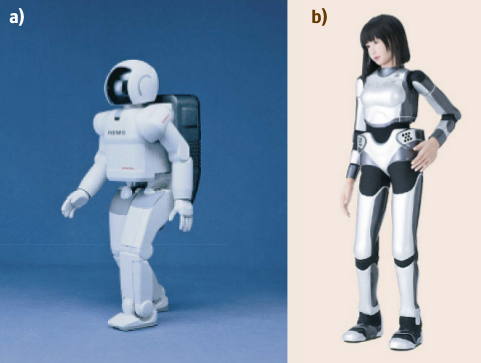
\includegraphics[scale=0.5]{images/asimov_and_HRP-4C.png}
	\caption{Ejemplos de robots humanoides (a) Asimov (2000); (b)HRP-4C (2009) (Tomado de: Siciliano and Khatib, 2016).}		
\label{fig:humanoids}%(Ver página 423).
\end{figure}



\subsection{Modelado y Control de Robots con Piernas}
	\textbf{Una Breve Historia de los Robots con piernas}\\
		Los robots con piernas controlados digitalmente empezaron a aparecer a finales de los 1960's. Entre los pioneros, Robert McGhee inicializó una serie de robots cuadrúpedos y hexápodos en \textit{University of South California}.\\

	\textbf{Dinámica del movimiento de los sistemas con piernas}\\
Como ya se había dicho con anterioridad, las mayores dificultades para hacer que un robot camine o corra es mantener su balance, de esta forma suelen formularse las siguientes preguntas: ¿Dónde debería caminar el robot?, ¿Cómo debería moverse su cuerpo a fin de moverse de manera segura en una dada dirección, incluso si hay fuertes perturbaciones?.\\ 

	\textbf{Análisis de estabilidad}\\
Para el control del sistema dinámico no lineal hay  un número de conceptos relativos para su seguridad y estabilidad:

\begin{itemize}
\item \textit{Puntos fijos} : Representan las posturas estáticas en cuáles el robot puede estar de pie de manera segura.

\item \textit{Ciclos límites}: Proveen una natural extensión del análisis de los puntos fijos para movimientos de caminata periódica.

\item \textit{Viabilidad}: La viabilidad es un concepto de invarianza controlada, que analiza el conjunto de estados del cual el robot es capaz de mantenerse de pie. Desafortunadamente esta propiedad puede ser intratable para el cómputo.

\item \textit{Controlabilidad}: La controlabilidad provee una ligera noción de restricción de viabilidad, analizando el conjunto de estados del cual el robot es capaz de retornar a un particular punto fijo.

\item \textit{Estabilidad robusta}: Examina las propiedades del sistema considerando el "peor de los casos" de las perturbaciones. Por instancias, un controlador robusto debería ser capaz de garantizar que un punto fijo es estable incluso si la estimación de masa del tronco tiene un error del $\pm$10\%.

\item \textit{Estabilidad estocástica}: El análisis estocástico provee herramientas para investigar la probabilidad de caer. Para muchos modelos de perturbaciones en robots el sistema caerá eventualmente (con probabilidad uno), pero el análisis puede revelar la distribución del tiempo de vida metaestable.

\item \textit{Estabilidad de entrada-salida}: En este análisis se trata una particular perturbación como una entrada, un criterio de rendimiento como salida e intenta calcular una ganancia relativa o sensibilidad del rendimiento del robot debido a esta entrada.

\item \textit{Márgenes de estabilidad}: El análisis de robustez puede ser difícil. En la práctica, los diseñadores del control a menudo se conforman con que el sistema se mantenga cómodamente lejos de los límites de estabilidad determinista.		

\end{itemize}
%	\section{Aplicaciones en el juego de Futbol Soccer}
%	\section{Conceptos básicos de visión computacional}
%	\section{El filtro de Kalman}
%	\section{Trabajo relacionado}		
\chapter{ Segmentación de imágenes con base en color}
\section{Modelo de cámara Estenopeica \textit{(Pinhole)}}
De acuerdo con \cite{bradski2008learning} la visión es la detección de la luz del mundo. El proceso de visión empieza cuando un rayo de luz es emanado desde una fuente hacia un objeto. Cuando la luz choca con el objeto, mucha de esta luz es absorbida, la que no, se puede percibir como el color, de esta manera, la luz reflejada hace su camino hacia el sensor óptico.

El modelo más simple de cómo sucede la captura de luz, es el de la cámara estenopeica o \textit{pinhole}. Una cámara estenopeica se puede imaginar como una habitación sin ventanas en donde la luz únicamente entra por una pequeña apertura en el centro de la pared proyectando así una imagen dentro de la habitación. Véase la Figura(\ref{fig:pinholeCamera}).

\begin{figure}
	\centering		
	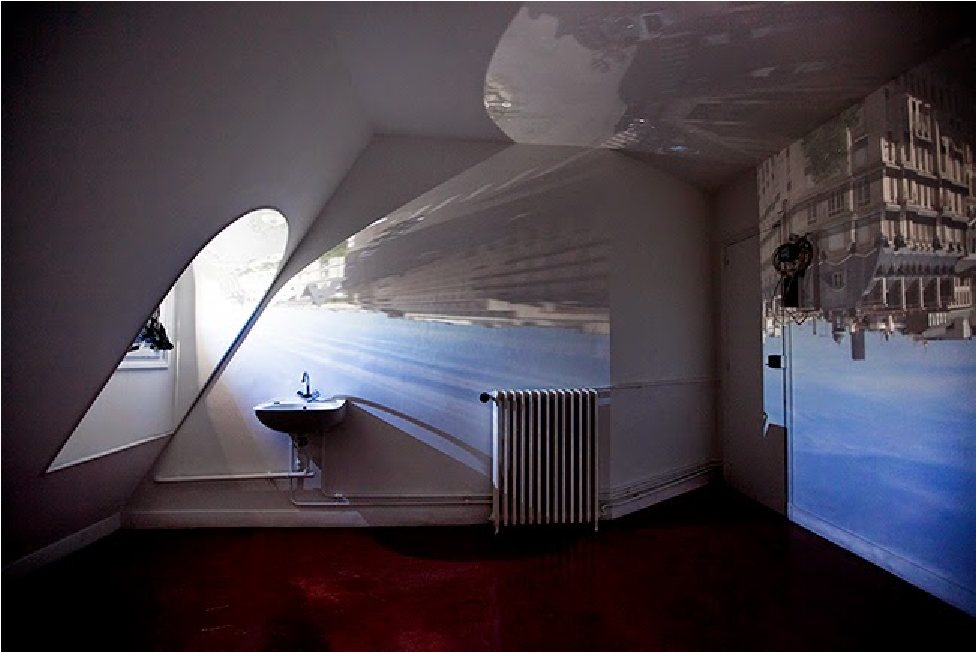
\includegraphics[scale=0.7]{images/pinholeCamera.pdf}
	\caption{Ejemplo en la vida real de la proyección de una imagen con la cámara estenopéica (Tomada de: https://www.pinterest.com.mx/pin/371828512962028619/).}		
	\label{fig:pinholeCamera}
\end{figure}

En la cámara estenopeica se considera que sólo un rayo de luz entra desde un punto en particular, este punto es luego \textit{proyectado} sobre una superficie generalmente plana. Como resultado, la imagen en este plano (también llamado plano proyectivo), está siempre en el foco y su tamaño se relaciona a la distancia del objeto por un sólo parámetro: \textit{la distancia focal}. La principal diferencia entre la imagen real y la que aparece en una cámara Pinhole, es que la imagen aparece invertida. 
	
El punto dentro del Pinhole es reinterpretado como el centro de proyección. Para este tipo de cámara, la distancia desde la abertura del Pinhole hacia la pantalla, es precisamente la distancia focal. Como puede verse en la Figura \ref{fig:pinholeScheme}.\\
	
\begin{figure}
	\centering		
	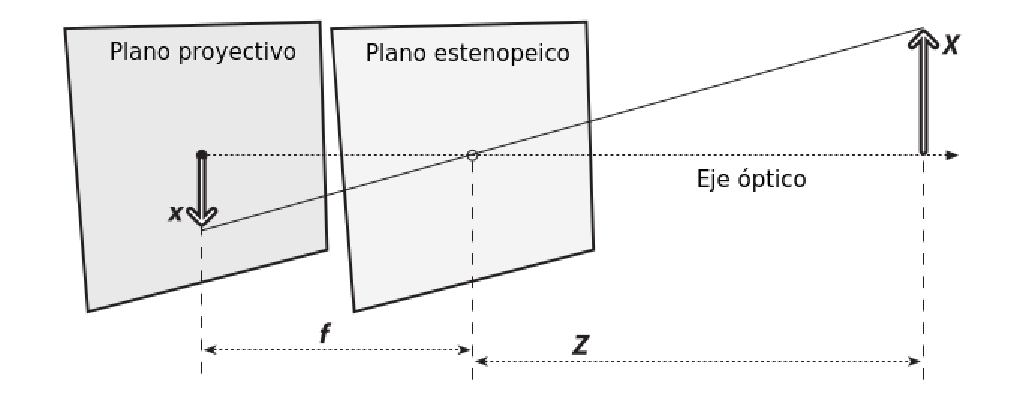
\includegraphics[scale=0.8]{images/pinholeScheme.pdf}
	\caption{Esquema del modelo de cámara estenopeica (Modificado de: Bradski and Kaehler, 2008).}		
	\label{fig:pinholeScheme}
\end{figure}

En la Figura(\ref{fig:pinholeScheme}), $f$ es representada como la distancia focal de la cámara, $Z$ es la distancia de la cámara al objeto, $X$ es la longitud del objeto, y $x$ es la longitud de la la imagen proyectada en el plano. Dentro de la figura, se pueden ver dos triángulos semejantes de los cuales se puede deducir la siguiente expresión:
\[x = -f \frac{X}{Z}\]
	
Para fines prácticos, el modelo \textit{Pinhole} no es conveniente de usar en exposiciones rápidas, ya que toda su luz proviene de un solo punto. A fin de obtener otro modelo de cámara que recopile mayor cantidad de luz y tenga ecuaciones similares, pero sin signos negativos (correspondientes a la inversión de la imagen) se propone hacer un rearreglo en el que se coloca al frente del centro de proyección el plano proyectivo. Tal y como se ve en la Figura \ref{fig:rearrange_pinhole_scheme}.
	
\begin{figure}
	\centering
	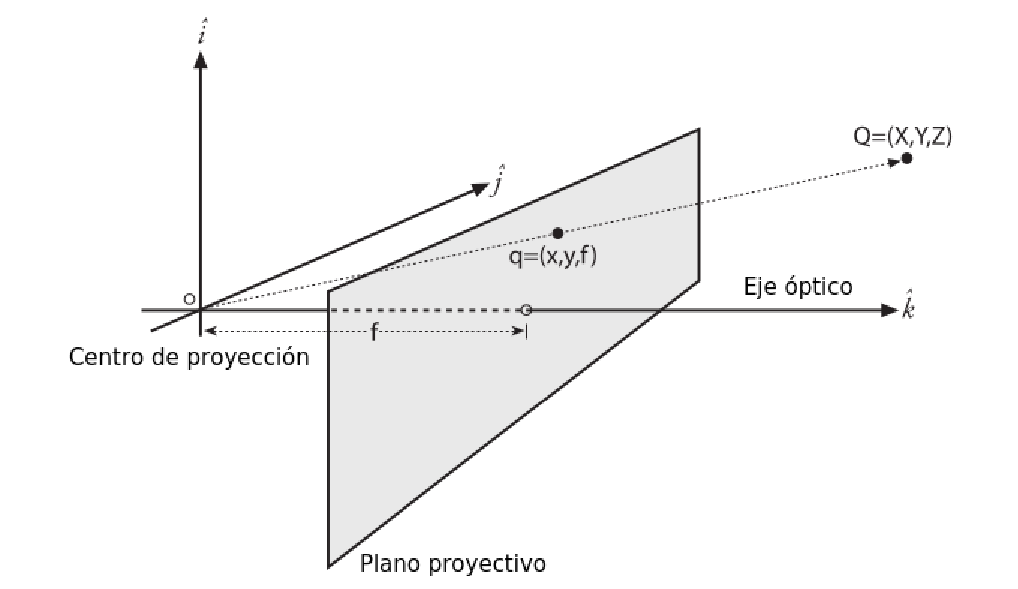
\includegraphics[scale=0.8]{images/rearrange_pinhole_scheme.pdf}
    \caption{Rearreglo de una cámara estenopeica (Modificado de: Bradski and Kaehler, 2008).}
    \label{fig:rearrange_pinhole_scheme}
\end{figure} 

Con este nuevo cambio, cada rayo de luz proveniente del objeto distante se dirije hacia el \textit{centro de proyección} y deja un punto en el \textit{plano proyectivo}. El punto de intersección del plano proyectivo y el eje óptico es conocido como \textit{el punto principal}. La imagen proyectada en este nuevo plano de imagen, tiene exactamente el mismo tamaño que en el esquema mostrado en la Figura(\ref{fig:pinholeScheme}) pero en este caso, la imagen no queda invertida, por lo que su relación de triángulos quedaría de la siguiente manera: 

\[\frac{x}{f} = \frac{X}{Z}\]

Se podría pensar que que \textit{el punto principal} es equivalente al centro de la imagen, sin embargo, este centro usualmente no está en el eje óptico, es por eso que se introducen dos nuevos parámetros, $c_{x}$ y $c_{y}$ para modelar un posible desplazamiento (perpendicular al eje óptico) del centro de coordenadas en el plano de proyección. El resultado es que un punto $Q$ en el mundo físico cuyas coordenadas son  (X,Y,Z) es proyectado dentro de la pantalla en una localización de pixeles dada por $(x_{screen},y_{screen})$ de acuerdo con las siguientes ecuaciones:

\[x_{screen}=f_{x}\left(\frac{X}{Z}\right ) + c_{x}\]	
\[y_{screen}=f_{y}\left(\frac{Y}{Z}\right ) + c_{y}\]

Nótese que se han introducido dos diferentes distancias focales $f_{x}$ y $f_{y}$, la razón es porque generalmente los pixeles son rectangulares.
		
\section{Corrección de la distorsión}

\subsection{Geometría básica proyectiva}
La relación que mapea los puntos $Q_{i}$ en el mundo físico con coordenadas $(X_{i},Y_{i},Z_{i})$ a los puntos en el plano de proyección con coordenadas $(x_{i},y_{i})$ es llamada una \textit{transformación proyectiva}. Cuando se trabaja con estas transformaciones es conveniente usar las \textit{coordenada homogéneas}. El plano de imagen es el espacio proyectado y tiene dos dimensiones, con lo que se pueden representar puntos en el plano como un vector tridimensional $q=(q_{1},q_{2},q_{3})$ ó $q=(x, y, w)$, en donde w es la orientación. Una forma de hacer un arreglo con los parámetros que definen a la cámara $f_{x},f_{y},c_{x}$ y $c_{y}$ dentro de una matriz de 3x3 es la llamada \textit{matriz de parámetros intrínsecos}. La proyección $q$ de los puntos del mundo físico en el plano de la imagen se puede calcular como: 
\[q=MQ\]
donde
\[q=
\begin{bmatrix}
x\\ 
y\\
w 
\end{bmatrix}\;,\;M=
\begin{bmatrix}
f_{x} & 0 & c_{x}\\ 
0     &f_{y}&c_{y} \\
0     & 0 & 1
\end{bmatrix}\;,\;Q=
\begin{bmatrix}
X\\
Y\\
Z
\end{bmatrix}
\]
\subsection{Distorsión de las lentes}

Debido a diversos factores en la manufactura, las lentes de una cámara no son perfectas, y al obtener una imagen, esta puede notarse distorsionada (véase la Figura \ref{fig:image_distorted}). La distorsión es un fenómeno que todas las cámaras tienen, no obstante, es más evidente en las cámaras de baja calidad o en las que tienen lentes tipo \textit{ojo de pescado}. Las distorsiones más características son: las \textit{Distorsiones radiales} y las \textit{Distorsiones tangenciales}. Las primeras surgen como resultado de la forma de las lentes y las segundas como resultado del proceso de ensamblado de la cámara.

\begin{figure}
\centering
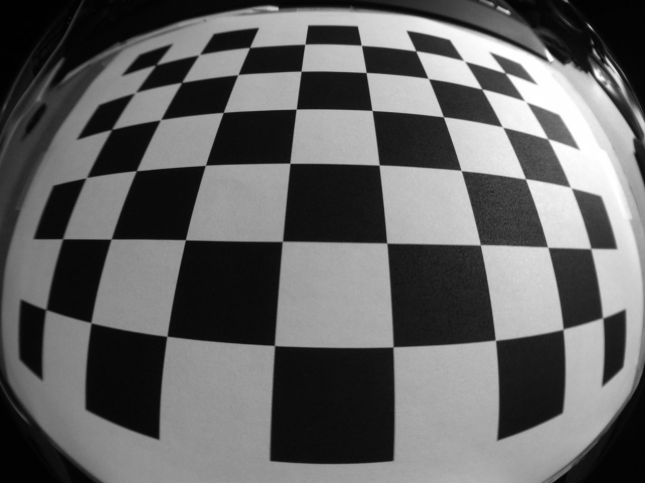
\includegraphics[scale=0.5]{images/image_distorted.png}
\caption{Ejemplo de distorsión de una cámara.}
\label{fig:image_distorted}
\end{figure}

Cuando la imagen se hace más pequeña conforme está más cerca de los bordes se está viendo una \textit{distorsión radial} (véase la figura \ref{fig:radial_distortion}). En la práctica, se puede caracterizar con la serie de Taylor, las ecuaciones son:
\[x_{corregida} = x(1+k_1r^2+k_2r^4+k_3r^6)\]
\[y_{corregida} = y(1+k_1r^2+k_2r^4+k_3r^6)\]

En donde $(x,y)$ son las coordenadas de la imagen, \textit{r} es la distancia del punto de la imagen al centro y las constantes $k_1$, $k_2$ y $k_3$ son parámetros que están relacionados a cada cámara en específico.

\begin{figure}
\centering
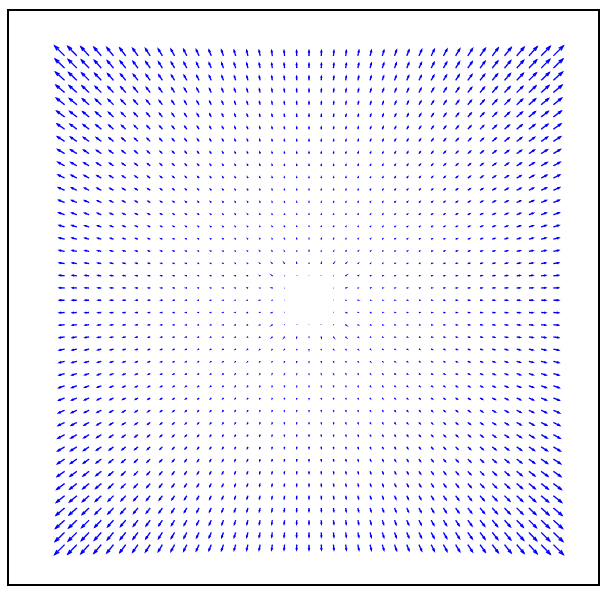
\includegraphics[scale=0.7]{images/radial_distortion.png}
\caption{Distribución de la distorsión radial de una imagen.}
\label{fig:radial_distortion}
\end{figure}

Las \textit{Distorsiones tangenciales} son ocasionadas por no tener paralelas las lentes con el plano de la imagen, vea la distribución de la distorsión tangencial en la figura \ref{fig:tangential_distortion}. Para obtener expresiones que ayuden a corregir este tipo de distorsión se introducen dos parámetros: $p_{1}$ y $p_{2}$ dentro de las siguientes ecuaciones:
\[x_{corregida} = x + [2p_1y+p_2(r^2+2x^2)]\]
\[y_{corregida} = y + [p_1(r^2+2y^2)+2p_2x]\]

La estimación de los parámetros internos es importante en la calibración de las cámaras, de esto depende la exactitud de las mediciones de distancia dadas por la visión computacional. \cite{bradski2008learning}.

\begin{figure}
\centering
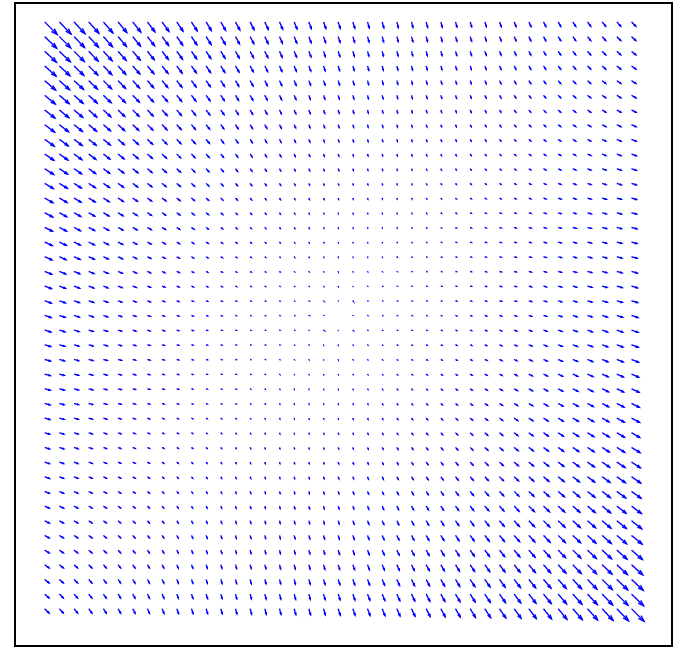
\includegraphics[scale=0.7]{images/tangential_distortion.png}
\caption{Distribución de la distorsión tangencial en una imagen.}
\label{fig:tangential_distortion}
\end{figure}

Para poder hacer una corrección automática de todas las distorsiones, las herramientas de OpenCV (véase la sección 5.2) usan los cinco parámetros antes mencionados dentro de una matriz de 1x5 llamada \textit{matriz de coeficientes de distorsión}, en donde cada parámetro se acomoda de la siguiente forma:
\[[k_1 \quad k_2 \quad p_1 \quad p_2 \quad k_3]\]


\section{Los espacios de color RGB y HSV}
El el pocesamiento de imágenes se usa el color debido a que es un buen descriptor para la identificación de objetos (mejor que otro tipo de segementación como el de escala de grises) \cite{gonzalez2002digital}.

\textbf{Percepción del color}\\
Según \cite{agoston2005computer} en el caso más simple, la percepción del color tiene tres características principales llamadas \textit{matiz, saturación y brillo}. 
\begin{itemize}
\item \textit{Matiz (Hue):} La matiz es un descriptor de qué tan combinados están los colores unitarios entre sí (si se entiende por color unitario a los colores rojo, amarillo, verde y azul).

\item \textit{Saturación (Saturation): } La saturación es la percepción de la relativa carga de color que tiene la matiz. Se puede decir que la saturación es una medida de qué tan puro es un color si éste es diluido en blanco.

\item \textit{Brillo: (Brightness)} El brillo es un atributo de la iluminación en la cual un objeto no aislado se ve afectado, es notable cuando un objeto de un  mismo color cambia su tonalidad debido a las variaciones de iluminación de su entorno.
\end{itemize}

\textbf{Espacios de color}
El \textit{espacio de color} es un modelo utilizado para facilitar la especificación de cualquier color de una manera estandarizada. Uno de los sistemas más conocidos, es el espacio de color RGB (por sus siglas en inglés red, green y blue), que está basado en un sistema coordenado ortogonal (como se observa en la Figura 2.3) en donde la escala de los colores primarios está cada uno en los ejes.

El espacio de color \textit{HSV (Hue-Saturation-Value)} es especificado por por tres números que corresponden a la matiz (Hue), saturación (saturation) y el valor (value). La matiz corresponde a un ángulo de 0 a 360 grados. La saturación se toma entre valores de 0 a 1 que miden la salida de la matiz del blanco. El valor (value) que va del 0 al 1 mide la salida de la matiz del negro o \textit{color de energía cero}, véase la Figura 2.4 en donde se observa el modelo tridimencional de este espacio.

\begin{figure}
	\centering		
	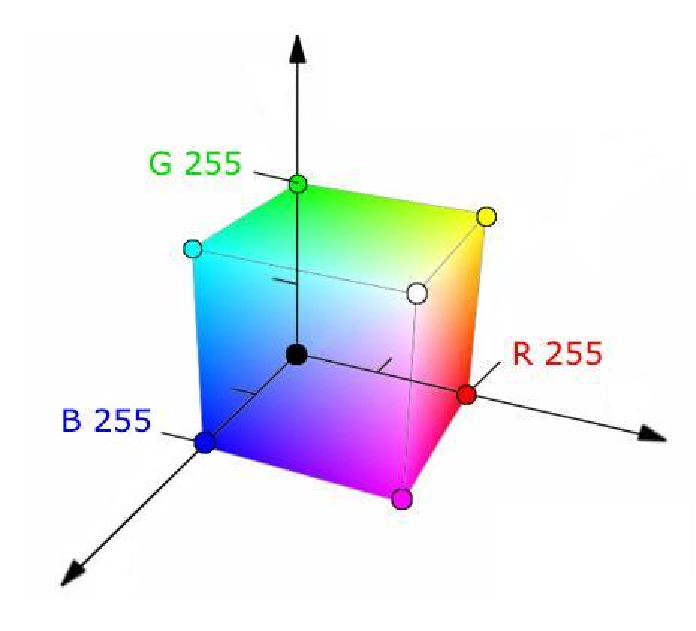
\includegraphics[scale=0.8]{images/RGB_model.pdf}
	\caption{Modelo tridimensional del espacio de color RGB (Foto tomada de: ).}		
\end{figure}

\begin{figure}
	\centering		
	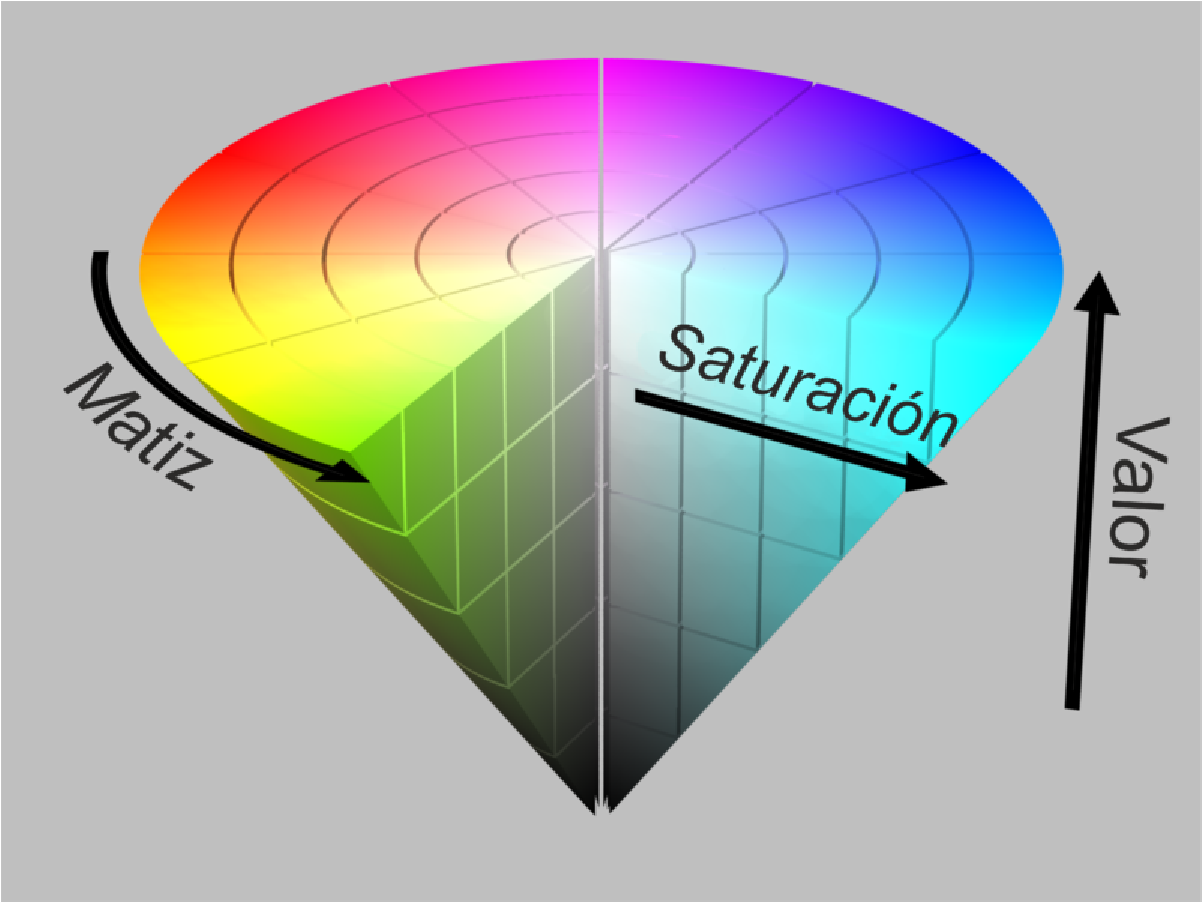
\includegraphics[scale=0.5]{images/hsv_space.pdf}
	\caption{Modelo tridimensional del espacio de color HSV (Foto tomada de: \cite{agoston2005computer}).}		
\end{figure}

Tanto el espacio de color RGB y el HSV pueden representar la totalidad de los colores del espectro de luz visible, no obstante para el procesamiento de imágenes se utiliza el HSV ya que es una forma más sencilla para segmentar colores y es una forma más parecida a la que los seres humanos percibimos los colores.

\section{Operadores morfológicos}	
La gran mayoría de las veces, cuando se hace procesamiento de imágenes, se necesitan ciertos procesos para eliminar el ruido circundante y dejar al elemento de interés aislado. Los \textit{operadores morfológicos} (erosión y dilatación) se pueden usar para este propósito.

Los \textit{operadores morfológicos} son operadores matemáticos basados en la forma de una imagen comunmente binaria (con pixeles blancos y negros) y sirven para preservar sus características y eliminar las irrelevancias. Dado que toda imagen está compuesta por pixeles, se pueden crear ciertos conjuntos de pixeles dentro de un vector para así poder aplicar operaciones matemáticas. 

La \textit{erosión} es el primer operador que se aplica cuando se desea eliminar el ruido en una segmentación, eso es porque elimina una gran cantidad de pixeles que tienden a tener mucha menor área que la figura de interés. Para lograr esto se establecen dos conjutos (de coordenadas de pixeles) $A$ y $B$. Si $A$ y $B$ son conjuntos dentro de un espacio euclidiano de N elementos, entonces la erosión de $A$ por $B$ es el conjunto de elementos $x$ para el cual $x + b \in  A$ para cada $b \in B$. Entonces, de una manera más formal, la operación de erosión se puede definir con la expresión \ref{eq:erosion}.
En la figura \ref{fig:erosion_diagram} se puede observar de una manera más visual cómo funciona la operación de erosión dentro de una imagen binaria.
\begin{equation}
A\thinspace\ominus\thinspace B\thinspace=\thinspace \left \{ x \in E^N  \mid x+b \in A \enspace \forall \; b \in B\right \}
\label{eq:erosion}
\end{equation}

 Para entender de mejor manera cómo es esta operación se debe entender lo que es un \textit{kernel}. Un \textit{kernel} es un conjunto de pixeles de cualquier forma o tamaño que se caracteriza por tener un pixel de anclaje dentro de sí (en la figura \ref{fig:erosion_diagram} es el pixel con un punto blanco). En el ejemplo de la figura \ref{fig:erosion_diagram} se le llamará \textit{kernel} al conjunto $B$ y siempre debe ser de menor tamaño que el conjuto $A$. La intersección del conjunto $A$ con el $B$ al ir colocando el pixel de anclaje en cada pixel del conjunto $A$ es la imagen resultante para la erosión.
 
\begin{figure}
\centering 
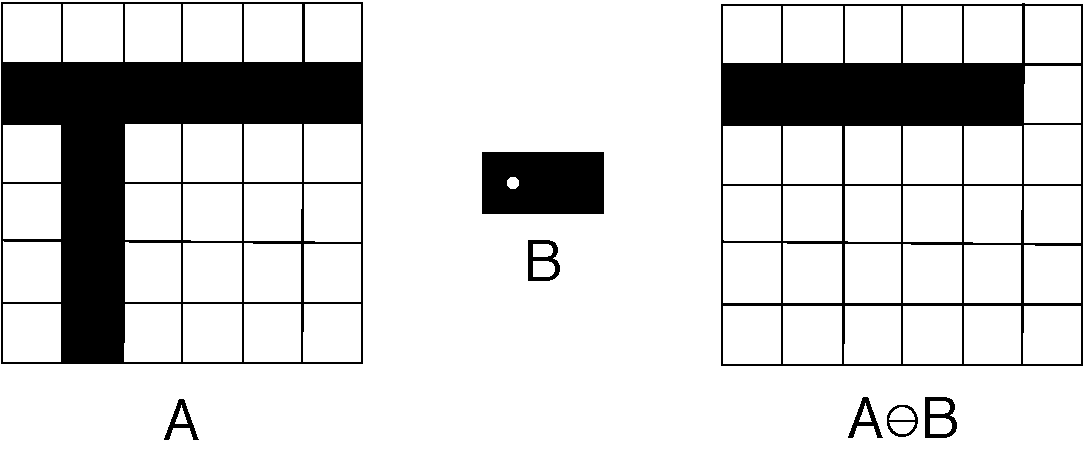
\includegraphics[scale=0.7]{images/erosion_diagram.pdf}
\caption{Ejemplo de la operación de erosión en una imagen binaria.}
\label{fig:erosion_diagram}
\end{figure}

En la figura \ref{fig:erosion_example} se ve que la erosión ha eliminado el ruido y la imagen se ve más limpia de puntos blancos que rodean la región de interés. El problema de hacer este procedimiento es que la imagen original suele verse afectada y tiende a encogerse o a deformarse, esto puede representar un problema para la detección de contornos. Para solucionarlo se procede a aplicar una operación opuesta a la erosión, mejor conocida como \textit{dilatación}.

Una vez eliminado el ruido gracias a la erosión, la \textit{dilatación} procede a ensanchar la figura de interés utilizando la adición de dos conjuntos de elementos. De la misma manera en que se hizo la erosión se procede a nombrar dos conjuntos $A$ y $B$. Si $A$ y $B$ son conjuntos dentro de un espacio euclidiano de N elementos. Sean $a \in A$ y $b \in B$ en donde $a=(a_1, ... ,a_n)$ y $b=(b_1,...,b_n)$, es decir conjuntos con coordenadas de pixeles, entonces la dilatación de $A$ por $B$ es el conjunto de todas las posibles sumas de elementos, de $A$ y $B$. De forma formal \ref{eq: dilation}:
\begin{equation}
A\thinspace\oplus\thinspace B\thinspace=\thinspace \left \{ c \in E^N  \mid c=a+b \quad\forall \quad a \in A \; y\; \; b \in B\right \}
\label{eq: dilation}
\end{equation}


\begin{figure}
\centering
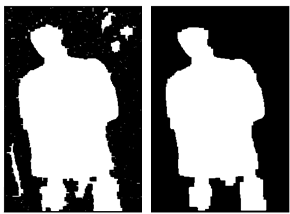
\includegraphics[scale=1]{images/erosion_example.png}
\caption{Eliminación de ruido alrededor de una figura de interés usando la erosión.}
\label{fig:erosion_example}
\end{figure}

En la figura \ref{fig:dilation_diagram} se puede imaginar que si se coloca el \textit{kernel} dentro de los pixeles pertenecientes al conjunto $A$ y se suman, queda como resultado de $A \oplus B$ una imagen ensanchada, lo que puede ayudar a que la figura erosionada tenga mayor parecido a la imagen original \cite{4767941}. En la figura \ref{fig:dilation_example} está ya un ejemplo de cómo se ensancha una figura al aplicar la dilatación.

\begin{figure}
\centering
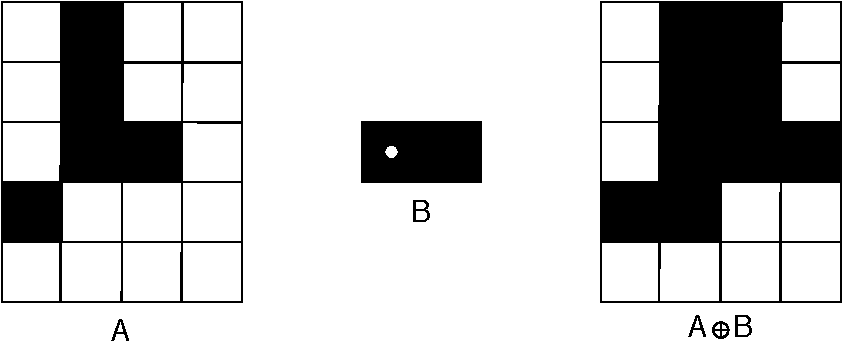
\includegraphics[scale=1]{images/dilation_diagram.pdf}
\caption{Ejemplificacion de la operación de dilatación en una imagen binaria.}
\label{fig:dilation_diagram}
\end{figure}

\begin{figure}
\centering
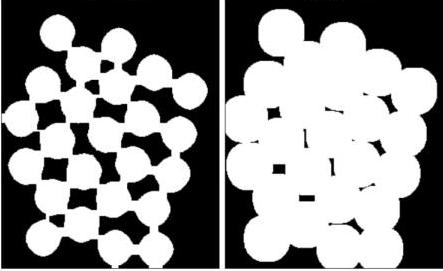
\includegraphics[scale=0.7]{images/dilation_example.jpg}
\caption{Ejemplificación de la dilatación aplicada en una segmentación de color.}
\label{fig:dilation_example}
\end{figure}

\chapter{Estimación de posición y velocidad}
	\section{Cálculo de la posición del objeto de interés}
Tal como se observa en la simulación de Gazebo (Figura 3.1), se decidió usar un sistema ortogonal derecho en la base de los pies como sistema de referencia que gobernará a todo el modelo.

\begin{figure}
	\centering		
	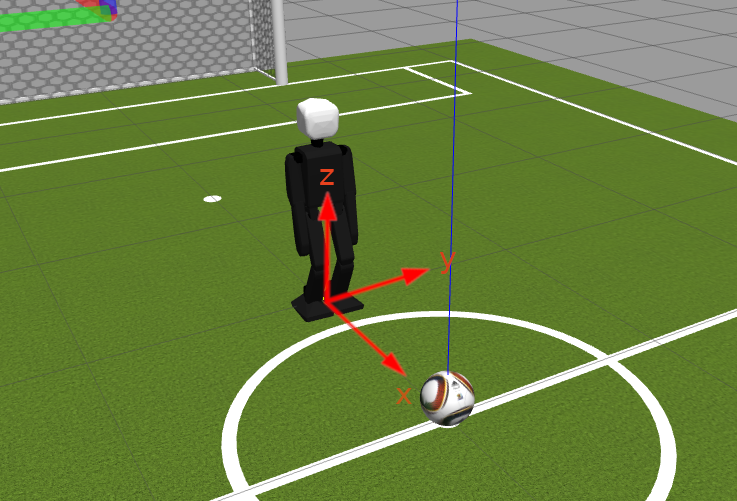
\includegraphics[scale=2]{images/robot_ejes.png}
	\caption{Representación del sistema de referencia usado en el robot.}		
\end{figure}

La cámara está localizada en la cabeza del humanoide, por lo que su centro
de visión se puede representar por un eje que va de la cámara al centroide del 
objeto, en este caso un balón de fútbol.
Para estimar la posición de un objeto que cruce por el centro de visión de la
cámara se necesita establecer un vector unitario:
\[\hat{u} = (u_x, u_y, u_z)\]
conocido en computación gráfica como vector \textit{look at}, (ver figura \ref{fig:LookAt}). Para obtener la ecuación vectorial de la recta paralela al vector \textit{look at} se toma un punto que contenga la recta, en este caso la posición de la cabeza en donde se encuentra la cámara: 

\begin{figure}
	\centering		
	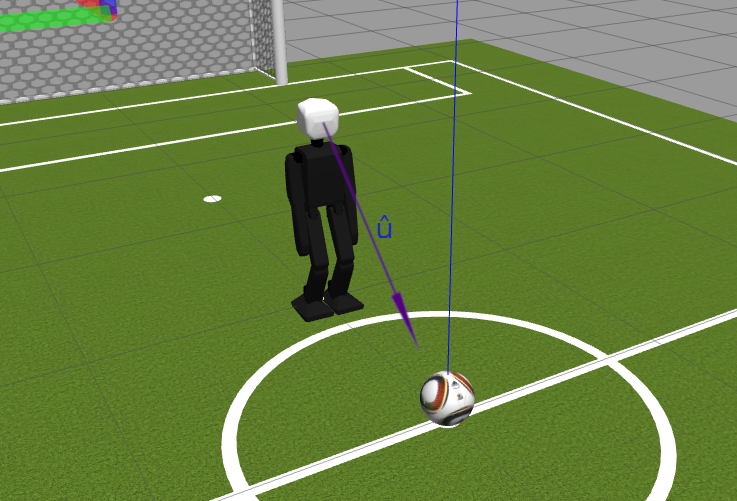
\includegraphics[scale=2]{images/robot_lookat.png}
	\caption{Representación del vector \textit{look at} utilizado en visión computacional.}		
	\label{fig:LookAt}
\end{figure}

\begin{equation}
\label{eq:LookAt}
r(\lambda) = (r_x, r_y, r_z)\quad +\quad \lambda (u_x, u_y, u_z)
\end{equation}


En donde $(r_x, r_y, r_z)$ es la posición en el espacio de la cámara utilizada, referida al sistema de referencia anteriormente mencionado. Se considera que el objetivo siempre estará en el suelo, por lo que el punto de intersección de la ecuación de la recta con el suelo hacen que la variable de altura sea igual a cero, conforme a la siguiente expresión:
\[r = (x, y, 0) = (r_x, r_y, r_z) + \lambda (u_x, u_y, u_z)\]
Despejando $\lambda$ del tercer término de la expresión anterior se obtiene:
\[\lambda = -\frac{r_z}{u_z}\]

De esta manera, substituyendo $\lambda$ en (\ref{eq:LookAt}), se obtiene:
\[x = r_x-\frac{r_z u_x}{u_z}\]
\[y = r_y-\frac{r_z u_y}{u_z}\]

Ya teniendo estas expresiones se procede a sustituir al vector unitario \textit{look at} con coordenadas esféricas, tal y como se observa en la siguiente expresión:
\begin{equation}
\label{eq:LookAtUnitary}
\hat{u}=(u_x, u_y, u_z)=(\sin{ \theta}\cos{\varphi},\sin{\theta}\sin{ \varphi},\cos{\theta})
\end{equation}

Sustituyendo la expresión (\ref{eq:LookAtUnitary}) dentro de los valores $x$ y $y$ quedan como:
\[x=r_x - \frac{r_z \sin{ \theta} \cos{\varphi}}{\cos{\theta}}\]
\[y=r_y - \frac{r_z \sin{\theta} \sin{ \varphi}}{\cos{\theta}}\]

Utilizando la identidad trigonométrica:
\[\tan{\theta} = \frac{\sin{\theta}}{\cos{\theta}}\]

Las ecuaciones para obtener la posición del objetivo siempre y cuando $z=0$ quedan:
\begin{equation}
\label{eq:xBidimentionalPosition}
x=r_x - r_z \tan{\theta}  \cos{\varphi}
\end{equation}

\begin{equation}
\label{eq:yBidimentionalPosition}
y=r_y - r_z \tan{\theta} \sin{\varphi}
\end{equation}

No obstante, el objeto a considerar no es un objeto bidimensional, es un balón con forma esférica que está sobre el plano del suelo, debido a esto se procede a hacer complementar las ecuaciones \ref{eq:xBidimentionalPosition} y \ref{eq:yBidimentionalPosition}, para obtener la posición (x,y,z) del centro del balón.

En la figura \ref{fig:ballProjection}(a) se observa un diagrama del balón en donde el vector \textit{look at} atravieza su centro e intersecta con el suelo en un punto en donde el balón no está. Esto representa un problema, ya que la posición en $x$ sufre una proyección, la cual incrementa mientras el balón tenga mayor radio. A esta proyección se le pondrá la variable $x_c$. Véase la figura \ref{fig:ballProjection}(b)


\begin{figure}
	\centering
	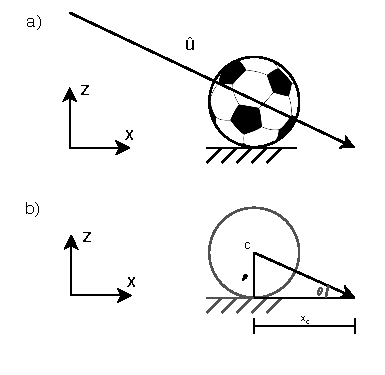
\includegraphics[scale=1.4]{images/ball_projection.pdf}
	\caption{(a) Bosquejo del vector \textit{look at} atravezando el centro del balón esférico; (b) Diagrama de la obtención de la distancia de proyección $x_c$.}
	\label{fig:ballProjection}
\end{figure}

Para obtener la magnitud de $x_c$ es necesario analizar el diagrama de la figura \ref{fig:ballProjection}(b), en donde $\theta$ es el ángulo \textit{pitch} y $\rho$ es el radio del balón. Así se puede obtener la siguiente igualdad:
\[\cot{\theta} = \frac{x_c}{\rho}\]\\

Despejando $x_c$
\[x_c = \rho \cot{\theta}\]

Debido a que $x_c$ se ve afectada también por la posición \textit{yaw} se deducen las siguientes igualdades para corregir el valor de la posición de $x$ y $y$ respectivamente:

\begin{equation}
\label{eq:xcForX}
x_{cx} = \rho \cot{\theta} \cos{\varphi}
\end{equation}

\begin{equation}
\label{eq:xcForY}
x_{cy} = \rho \cot{\theta} \sin{\varphi}
\end{equation}\\

De esta manera, se resta \ref{eq:xcForX}  a \ref{eq:xBidimentionalPosition} y \ref{eq:xcForY} a \ref{eq:yBidimentionalPosition}. Finalmente las ecuaciones resultantes son:

\[x = r_x - r_z \tan{\theta} \cos{\varphi} - \rho \cot{\theta} \cos{\varphi}\]
\[y = r_y - r_z \tan{\theta} \sin{\varphi} - \rho \cot{\theta} \sin{\varphi}\]
\[z = \rho \]

\chapter{Implementación}
\section{La plataforma ROS}
Citando a \cite{pyo2015ros} ROS es un meta sistema operativo \textit{open-source} que provee servicios a las aplicaciones de robótica, servicios que comunmente se esperan de un sistema operativo, tales como: abstracción de hardware, control de dispositivos a \textit{bajo nivel}, paso de mensajes entre procesos, ordenamiento y manejo de distintos tipos de paquetes. ROS también provee herramientas y bibliotecas para obtener, construir, escribir y ejecutar programas a través de multiples computadoras.\\

ROS es la abreviación en inglés de \textit{Robot Operating System} lo cual se prodría traducir al español como Sistema Operativo de Robots. Con este nombre se podría pensar que ROS es un sistema operativo, sin embargo el término mejor empleado es el de \textit{Meta Sistema Operativo}. Aunque \textit{Meta Sistema Operativo} no está definido en el diccionario, se puede describir como un sistema que realiza procesos tales como programación, ejecución, monitoreo, y manejo de errores, utilizando una capa de visualización entre aplicaciones y recursos informáticos distribuidos.\\

Dicho lo anterior, ROS no es un sistema operativo convencional, tal como \textit{Windows}, \textit{Linux}, o \textit{Android}, sino una plataforma que se ejecuta dentro del sistema operativo instalado. A menudo, para utilizar ROS se requiere tener instalado \textit{Ubuntu}, que es un sitema basado en las distribuciones de \textit{Linux}. No obstante, es posible usarse en distintos sitemas, tal y como se muestra la figura \ref{fig:meta_operating_system}. 
\begin{figure}
\centering
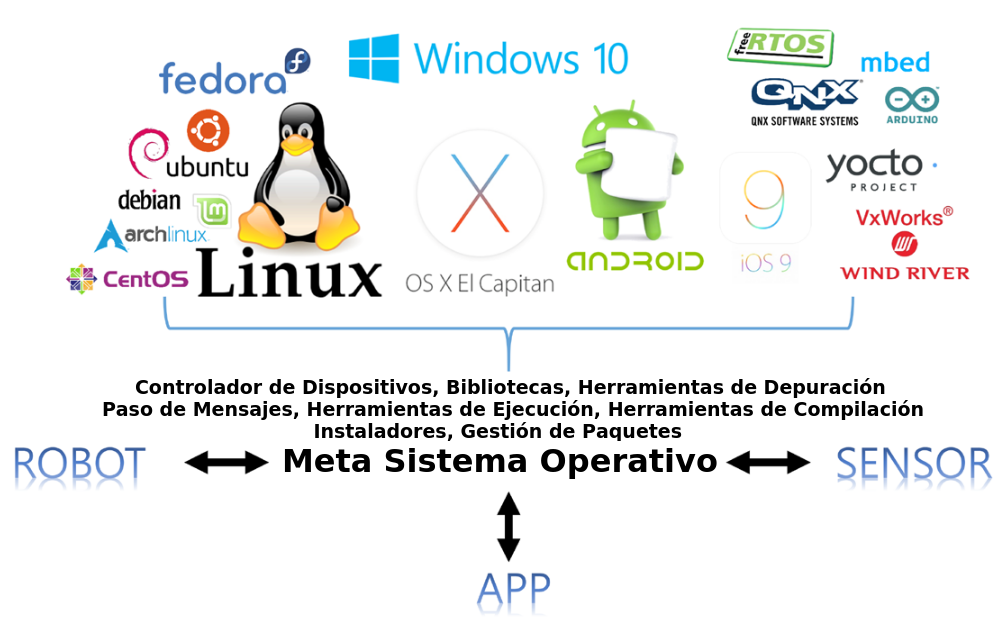
\includegraphics[scale=0.5]{images/meta_operating_system.png}
\caption{Esquema de la abstracción de harware por ROS en distintos Systemas Operativos}
\label{fig:meta_operating_system}
\end{figure} 

\subsection*{Objetivos al utilizar ROS}
Aunque existen diversas plataformas de robótica (OpenRTM, OPRoS, Player, Orca, Microsoft Robotics Studio, etc.), ROS está orientado a construir entornos de desarrollo para software de robótica a un nivel global, con esto se espera que el código de diferentes desarrolladores se pueda usar, modificar o mejorar para hacer crecer el entorno mismo. Para hacer de una manera sencilla el entorno de desarrollo, ROS tiene las siguientes características:

\begin{itemize}
\item \textbf{Distribución de procesos:}
Están programados en unidades mínimas de procesamiento (nodos). Cada uno de estos procesos se ejecuta de manera independiente y es capaz de intercambiar datos con otros de manera sistemática.  
\item \textbf{Manejo de paqueterías:}
Cuando varios procesos tienen propósitos similares, estos se manejan dentro de un \textit{paquete} que haga los procesos más ordenados y fáciles de desarrollar.
\item \textbf{Repositorios públicos:}
Cada paquete se hace público dentro de un repositorio (por ejemplo GitHub) para que la comunidad de desarrolladores puedan acceder a él. 
\item \textbf{API (Interfaz de Programación de Aplicaciones):}
Cuando se desarrolla un programa en ROS, generalmente se llaman funciones ya existentes fácilmente insertarlas dentro del código que se esté construyendo.
\item \textbf{Soporte de distintos lenguajes de programación:}
La plataforma ROS posee una \textit{bilioteca de clientes} para facilitar el trabajo de los programadores. La biblioteca puede importar lenguajes de programación que son bastantes populares, tales como Python, C++, Java, C#, Ruby, Lips, entre otros.
\end{itemize}
\subsection*{Breve historia de ROS}
\textit{Robot Operating System} fue creado en Mayo del 2007 por el Doctor Morgan Quigley (véase la figura \ref{fig:morga_quigley}) dentro del \textit{Standford Artificial Intelligence Laboratory}. Se podría decir que el predecesor de ROS es un proyecto llamado \textit{SwitchYard}, el cual es un programa creado por el mismo laboratorio para el desarrollo de inteligencia artificial.

En noviembre del 2007 la compañía estadounidense \textit{Willow Garage} empezó el desarrollo de ROS dentro del campo de los robots de servicio. De esta manera ROS vino al mundo oficialmente el 22 de Enero del 2010 con la versión llamada \textit{ROS 1.0}, sin embargo la versión más conocida fue \textit{Box Turtle} lanzada en Marzo del mismo año.

La plataforma ROS es actualizada cada dos años (entre el lapso de Abril-Octubre), lo que significa que cada versión tiene soporte durante la misma cantidad de tiempo. Para propósitos de esta tesis se optó por utilizar la versión \textit{ROS-Kinetic} instalado en Ubuntu 16.04 \textit{Xenial Xerus (LTS)}.
\begin{figure}
\centering
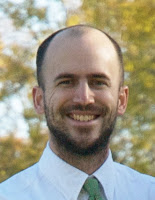
\includegraphics[scale=0.7]{images/morgan_quigley.jpg}
\caption{Dr. Morgan Quigley, uno de los principales fundadores de ROS. Imagen tomada de: https://web.stanford.edu/group/sailsbury_robotx/cgi-bin/salisbury_lab/?page_id=667}
\label{fig:morga_quigley}
\end{figure}


%	\chapter{Resultados}
\bibliographystyle{apacite}
%\bibliographystyle{ieeetr}
\bibliography{References}
\end{document}
